\subsection{Actividades Realizadas}

\subsubsection{Selección de Footprints}

Para comenzar el desarrollo de la PCB, primero se tomó la lista de componentes de la plataforma, provista por el programa, y se le asignó a cada uno de los componentes una \textit{footprint}, que es el patrón de pads (para dispositivos de montaje superficial o SMD) u orificios (para dispositivos de tecnología \textit{through-hole} o THT) de un componente sobre la superficie de la placa, sobre el cuál luego se suelda el componente apropiado.\\ 

Para esta plataforma se decidió utilizar, siempre que fuese posible, componentes de tipo SMD, ya que estos no atraviesan la placa y facilitan el ruteo de pistas de cobre al no ocupar espacio en la capa opuesta de la placa. Casi todas las resistencias y capacitores que se utilizan en la placa son de montaje superficial, de dimensiones 1206 (\SI[]{3}[]{\milli\metre} x \SI[]{1.5}[]{\milli\metre}), ya que es un tamaño bastante reducido que es fácil de conseguir en proveedores locales. En la figura \ref{fig:encapsulados} se puede ver este junto con otros encapsulados utilizados en la plataforma.\\

\begin{figure}[h]
    \centering
    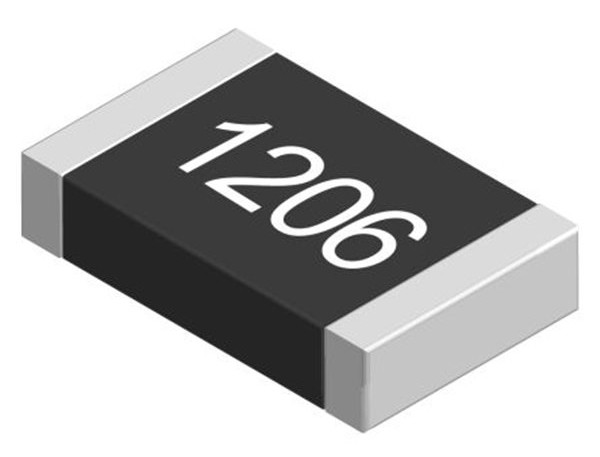
\includegraphics[scale=0.3]{Imagenes/1206.jpg}
    \caption{Algunos de los encapsulados que utilizan los componentes de la placa de circuito impreso (Placehoder: suponen ser varios encapsulados).}
    \label{fig:encapsulados}
\end{figure}

Para esto se comenzó utilizando la biblioteca de footprints y componentes disponible por defecto en el programa. Pero rápidamente se hizo claro que esto es insuficiente, por lo que se tuvo que recurrir a páginas web como \textit{SnapEDA}, que tiene un catálogo gratuito de footprints y símbolos esquemáticos para una enorme cantidad de componentes electrónicos.\\

\subsubsection{Posicionamiento y Conexión de Footprints}
 
\lipsum[1]\\

\subsubsection{Verificación del Diseño}
 
\lipsum[2]\\

\subsubsection{Contacto con Fabricantes}
 
\lipsum[3]\\